\documentclass[journal]{IEEEtran}
\IEEEoverridecommandlockouts

\usepackage{cite}
\usepackage{amsmath,amssymb,amsfonts,bm}
\usepackage[ruled,vlined,linesnumbered]{algorithm2e}
\usepackage{graphicx}
\usepackage{booktabs}
\usepackage{multirow}
\usepackage{tabularx}
\usepackage{textcomp}
\usepackage{xcolor}
\usepackage{tikz}
\usepackage{pgfplots}
\pgfplotsset{compat=1.18}
\usetikzlibrary{shapes.geometric, arrows.meta, positioning, fit, calc, backgrounds}

% Balanced float parameters for two-column layout
\setcounter{topnumber}{4}
\setcounter{bottomnumber}{4}
\setcounter{totalnumber}{8}
\setcounter{dbltopnumber}{4}
\renewcommand{\topfraction}{0.95}
\renewcommand{\bottomfraction}{0.95}
\renewcommand{\textfraction}{0.05}
\renewcommand{\floatpagefraction}{0.85}
\renewcommand{\dbltopfraction}{0.95}
\renewcommand{\dblfloatpagefraction}{0.85}

\def\BibTeX{{\rm B\kern-.05em{\sc i\kern-.025em b}\kern-.08em
    T\kern-.1667em\lower.7ex\hbox{E}\kern-.125emX}}

\begin{document}

\title{ReviTLS: Revision-Aware Timeline Summarization via Conditional Temporal Gating and Dual-Scale LLMs}

\author{Baran~G\"{u}\c{c}l\"{u}%
\thanks{Baran G\"{u}\c{c}l\"{u} is with the Department of Software Engineering, \.{I}n\"{o}n\"{u} University, Malatya, Turkey (e-mail: \texttt{36253632025@ogr.inonu.edu.tr}). Source code and evaluation scripts are publicly available at: \texttt{https://github.com/Baranll0/ReviTLS-Revision-Aware-Incremental-Timeline-Summarization}.}}

\markboth{IEEE TRANSACTIONS / JOURNAL SUBMISSION, 2026}%
{G\"{u}\c{c}l\"{u}: ReviTLS: Revision-Aware Timeline Summarization}

\maketitle

\begin{abstract}
Timeline summarization (TLS) condenses evolving news streams into chronologically ordered milestone summaries. Existing large language model (LLM) approaches implicitly assume that reported facts accumulate monotonically. In real-world breaking news, however, early numerical estimates, causal attributions, and unverified claims are frequently revised or retracted days later. Conventional same-day clustering prevents later corrections from updating earlier events, leaving outdated claims in the final summary; conversely, opening a multi-month matching window with larger LLMs induces cross-date over-merging that collapses distinct milestones. We present \textbf{ReviTLS}, a revision-aware framework that models events as mutable $5\text{W}1\text{H}$ state nodes equipped with explicit tombstone sets to purge superseded claims and filter retracted rumors. To balance temporal precision and long-range revision recall, ReviTLS combines a conditional dual-horizon temporal gate with cross-encoder reranking and a two-phase dual-LLM schedule (7B extraction followed by deferred 14B conflict verification). Across $13$ topics from Timeline17 and Crisis under identical local execution conditions, ReviTLS improves content coverage and alignment on Timeline17 over streaming baselines (e.g., Concat-R1 $0.400$ vs.\ $0.351$ for LLM-TLS), while offering smaller gains on denser Crisis streams and incurring roughly $4.5\times$ higher runtime due to structured extraction and verification. On $16$ controlled cross-domain revision scenarios and $8$ unseen fictional/counterfactual scenarios, ReviTLS resolves $81.3\%\text{--}87.5\%$ of revisions and $100\%$ of counterfactual controls with zero pre-correction leakage.
\end{abstract}

\begin{IEEEkeywords}
Timeline summarization, natural language processing, large language models, information retrieval, factual revision, rumor retraction.
\end{IEEEkeywords}

\section{Introduction}
\label{sec:intro}

\IEEEPARstart{C}{ondensing} massive, chronologically evolving document streams into concise summaries is a central challenge in natural language processing and information retrieval. Timeline summarization (TLS)~\cite{tran2013leveraging, martschat2018temporally, ghalandari2020examining} addresses this need by extracting pivotal events from a news collection and organizing them into a sequence of date-stamped milestone summaries. A high-quality timeline must simultaneously identify the exact dates on which key developments occurred (measured by $\text{Date-F1}$) and synthesize non-redundant, factually accurate descriptions for each selected date (measured by alignment-based ROUGE~\cite{martschat2017improving}).

Traditional TLS approaches formulate the task over a static document collection, employing submodular optimization~\cite{martschat2018temporally}, Markov clustering (\texttt{CLUST}) and supervised date selection (\texttt{Datewise})~\cite{ghalandari2020examining}, multi-timeline generation (\texttt{MTLS})~\cite{yu2021multi}, or event graph compression (\texttt{EGC})~\cite{li2021timeline}. Recently, Large Language Models (LLMs) have shifted the paradigm toward dynamic and incremental generation. Notably, Hu et al.~\cite{hu2024moments} proposed \textbf{LLM-TLS}, which treats an LLM as a pseudo-oracle to incrementally cluster incoming news events in a streaming setting before ranking milestone clusters via TextRank. Concurrently, Wu et al.~\cite{wu2025unfolding} introduced \textbf{CHRONOS}, an iterative retrieval-augmented generation (RAG) framework that poses $5\text{W}1\text{H}$ (\textit{Who, What, When, Where, Why, How}) self-questions to retrieve event passages and merge round-level timelines.

\begin{figure}[t]
\centering
\resizebox{\columnwidth}{!}{%
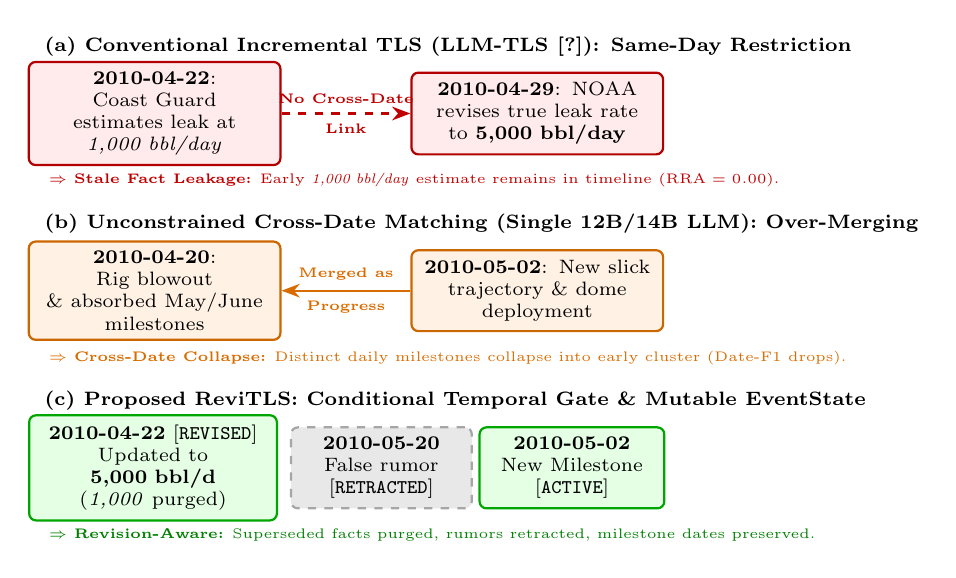
\begin{tikzpicture}[
    font=\scriptsize,
    box/.style={rectangle, rounded corners=2.5pt, draw=black!75, thick, inner sep=3.5pt, align=center},
    failbox/.style={box, fill=red!8, draw=red!70!black},
    warnbox/.style={box, fill=orange!10, draw=orange!80!black},
    okbox/.style={box, fill=green!10, draw=green!65!black},
    arrow/.style={-Stealth, thick}
]
% Panel A
\node[anchor=west, font=\scriptsize\bfseries] at (-0.1, 4.35) {(a) Conventional Incremental TLS (LLM-TLS~\cite{hu2024moments}): Same-Day Restriction};
\node[failbox, text width=2.95cm] (a1) at (1.42, 3.50) {\textbf{2010-04-22}: Coast Guard\\estimates leak at\\\textit{1,000 bbl/day}};
\node[failbox, text width=2.95cm] (a2) at (6.28, 3.50) {\textbf{2010-04-29}: NOAA\\revises true leak rate\\to \textbf{5,000 bbl/day}};
\draw[arrow, dashed, red!75!black] (a1) -- node[above, font=\tiny\bfseries] {No Cross-Date} node[below, font=\tiny\bfseries] {Link} (a2);
\node[anchor=west, font=\tiny, text=red!75!black] at (-0.05, 2.65) {$\Rightarrow$ \textbf{Stale Fact Leakage:} Early \textit{1,000 bbl/day} estimate remains in timeline ($\text{RRA}=0.00$).};

% Panel B
\node[anchor=west, font=\scriptsize\bfseries] at (-0.1, 2.10) {(b) Unconstrained Cross-Date Matching (Single 12B/14B LLM): Over-Merging};
\node[warnbox, text width=2.95cm] (b1) at (1.42, 1.25) {\textbf{2010-04-20}: Rig blowout\\\& absorbed May/June\\milestones};
\node[warnbox, text width=2.95cm] (b2) at (6.28, 1.25) {\textbf{2010-05-02}: New slick\\trajectory \& dome\\deployment};
\draw[arrow, orange!85!black] (b2) -- node[above, font=\tiny\bfseries] {Merged as} node[below, font=\tiny\bfseries] {Progress} (b1);
\node[anchor=west, font=\tiny, text=orange!85!black] at (-0.05, 0.40) {$\Rightarrow$ \textbf{Cross-Date Collapse:} Distinct daily milestones collapse into early cluster ($\text{Date-F1}$ drops).};

% Panel C
\node[anchor=west, font=\scriptsize\bfseries] at (-0.1, -0.15) {(c) Proposed ReviTLS: Conditional Temporal Gate \& Mutable EventState};
\node[okbox, text width=2.90cm] (c1) at (1.40, -1.00) {\textbf{2010-04-22} [\texttt{REVISED}]\\Updated to \textbf{5,000 bbl/d}\\(\textit{1,000} purged)};
\node[box, fill=gray!18, draw=gray!70, dashed, text width=2.05cm] (c2) at (4.30, -1.00) {\textbf{2010-05-20}\\False rumor\\{[\texttt{RETRACTED}]}};
\node[okbox, text width=2.10cm] (c3) at (6.72, -1.00) {\textbf{2010-05-02}\\New Milestone\\{[\texttt{ACTIVE}]}};
\node[anchor=west, font=\tiny, text=green!50!black] at (-0.05, -1.85) {$\Rightarrow$ \textbf{Revision-Aware:} Superseded facts purged, rumors retracted, milestone dates preserved.};
\end{tikzpicture}%
}
\caption{Comparison of incremental timeline summarization paradigms on evolving news streams. (a) Same-day clustering cannot link cross-date corrections and retains outdated claims. (b) Unconstrained cross-date matching over-merges distinct daily developments. (c) \textbf{ReviTLS} selectively gates cross-date retrieval for revision cues and updates mutable event states.}
\label{fig:paradigm}
\end{figure}

Despite their effectiveness on static narratives, current LLM-based TLS frameworks share a critical limitation: they assume that facts in a news stream accumulate monotonically without contradiction. In realistic streaming scenarios---such as industrial disasters (e.g., the 2010 Deepwater Horizon oil spill), public health emergencies, or financial crises---journalistic reporting is inherently non-monotonic and self-correcting:
\begin{enumerate}
    \item \textbf{Quantitative Revisions:} Preliminary estimates (e.g., an initial leak rate of ``1,000 barrels per day'' reported on April~22) are officially revised days later (``5,000 barrels per day'' on April~29).
    \item \textbf{Temporal and Causal Corrections:} Subsequent investigations reveal that an incident occurred on an earlier date than initially reported or overturn preliminary causal attributions.
    \item \textbf{Rumor Retractions:} Breaking reports of secondary incidents (e.g., an unconfirmed second pipeline breach) are later debunked by inspection teams and must be removed from the timeline.
\end{enumerate}

As illustrated in Fig.~\ref{fig:paradigm}(a), existing pipelines struggle with such updates. Because LLM-TLS~\cite{hu2024moments} restricts candidate matching to the same publication date and selects summary sentences via TextRank centrality, a correction published at $t + \Delta t$ cannot access the original cluster at $t$; moreover, heavily repeated early estimates outscore single authoritative corrections, resulting in severe \textit{Stale Fact Leakage}. Similarly, CHRONOS~\cite{wu2025unfolding} merges round-level timelines via surface-level deduplication without explicit conflict verification.

Crucially, our empirical analysis reveals a second challenge, which we term \textbf{Cross-Date Over-Merging} (Fig.~\ref{fig:paradigm}(b)). When the same-day constraint is relaxed to a multi-month lookback window (e.g., $90$~days) and paired with larger single-backbone LLMs, broader semantic associativity can cause subsequent daily developments within a single-topic stream to be misclassified as ongoing narrative updates of earlier clusters, collapsing distinct milestone dates into existing nodes.

To address both challenges, we propose \textbf{ReviTLS} (Fig.~\ref{fig:paradigm}(c)). Rather than treating event clusters as immutable bags of sentences, ReviTLS maintains a dynamic repository of mutable \texttt{EventState} nodes containing structured $5\text{W}1\text{H}$ slots, active and purged claim sets, and discrete lifecycle statuses (\texttt{ACTIVE}, \texttt{REVISED}, \texttt{RETRACTED}). To prevent cross-date over-merging while supporting long-range revisions, ReviTLS introduces a \textit{Conditional Dual-Horizon Temporal Gate} that enforces same-day matching for routine events while unlocking a 90-day lookback window coupled with cross-encoder reranking whenever revision cues are detected. Furthermore, a two-phase dual-LLM schedule pairs a $7\text{B}$ extractor in Phase~1 with deferred $14\text{B}$ conflict verification in Phase~2, minimizing GPU model-swapping overhead on consumer hardware.

Our study investigates three research questions: \textbf{RQ1:} Can conditional temporal gating resolve cross-date factual revisions and rumor retractions without sacrificing milestone date precision? \textbf{RQ2:} How do model scale, attention architecture, and timeline selection choices affect cross-date over-merging and revision accuracy? \textbf{RQ3:} Does revision resolution reflect in-stream evidence rather than parametric pretraining memorization?

Our main contributions are summarized as follows:
\begin{itemize}
    \item We formulate non-monotonic timeline summarization and propose \textbf{ReviTLS}, modeling events as mutable $5\text{W}1\text{H}$ state nodes governed by a four-way transition mechanism and explicit tombstone purging.
    \item We characterize \textit{Cross-Date Over-Merging} and address it through a Conditional Dual-Horizon Temporal Gate, hybrid cross-attention reranking, and a two-phase dual-LLM schedule ($7\text{B}$ extraction + deferred $14\text{B}$ verification).
    \item We provide a comprehensive empirical evaluation across $13$ standard TLS topics, $16$ multi-topic revision chains, and $8$ fictional/counterfactual controls under identical hardware constraints, alongside component ablations and failure analyses.
\end{itemize}

\section{Related Work}
\label{sec:related}

\subsection{Classical and Graph-Based Timeline Summarization}
Early research approached timeline summarization (TLS) over static document collections via three main paradigms~\cite{tran2013leveraging, tran2015timeline, martschat2017improving, ghalandari2020examining}: extractive optimization balancing salience and temporal diversity~\cite{martschat2018temporally}, supervised date selection coupled with per-date sentence compression (\texttt{Datewise})~\cite{ghalandari2020examining, steen2019abstractive}, and event clustering or graph compression (\texttt{CLUST}, \texttt{MTLS}, \texttt{EGC})~\cite{ghalandari2020examining, yu2021multi, li2021timeline}. While effective on static benchmarks, these offline methods require access to the entire document collection upfront and do not support incremental state revision.

\begin{figure*}[t]
\centering
\resizebox{\textwidth}{!}{%
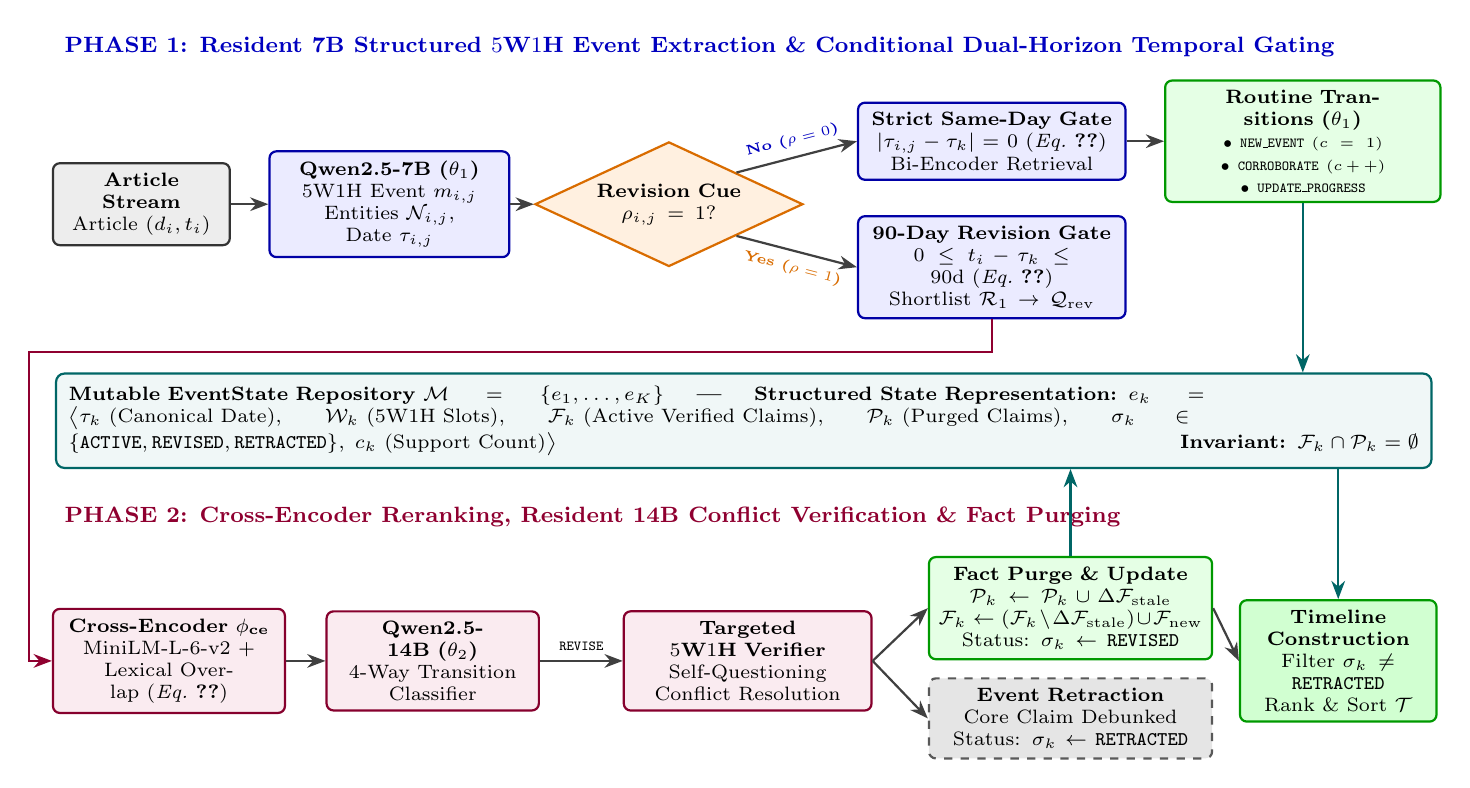
\begin{tikzpicture}[
    font=\scriptsize,
    block/.style={rectangle, rounded corners=2.5pt, draw=black!80, thick, minimum height=0.82cm, align=center, inner sep=3.5pt},
    phase1/.style={block, fill=blue!8, draw=blue!65!black},
    gate/.style={diamond, aspect=2.15, draw=orange!85!black, thick, fill=orange!12, align=center, inner sep=1.5pt},
    phase2/.style={block, fill=purple!8, draw=purple!70!black},
    state/.style={block, fill=green!10, draw=green!60!black},
    membox/.style={rectangle, rounded corners=3pt, draw=teal!80!black, thick, fill=teal!6, align=left, inner sep=4.5pt},
    retract/.style={block, fill=gray!20, draw=gray!70!black, dashed},
    arrow/.style={-Stealth, thick, draw=black!75}
]

% ================= PHASE 1 =================
\node[anchor=west, font=\footnotesize\bfseries, text=blue!75!black] at (-0.15, 6.45) {PHASE 1: Resident 7B Structured $5\text{W}1\text{H}$ Event Extraction \& Conditional Dual-Horizon Temporal Gating};

\node[block, fill=gray!14, text width=2.0cm] (stream) at (0.95, 4.45) {\textbf{Article Stream}\\Article $(d_i, t_i)$};
\node[phase1, text width=2.8cm] (extractor) at (4.10, 4.45) {\textbf{Qwen2.5-7B ($\theta_1$)}\\$5\text{W}1\text{H}$ Event $m_{i,j}$\\Entities $\mathcal{N}_{i,j}$, Date $\tau_{i,j}$};
\node[gate, text width=1.95cm] (revgate) at (7.65, 4.45) {\textbf{Revision Cue}\\$\rho_{i,j} = 1$?};

\node[phase1, text width=3.15cm] (sameday) at (11.75, 5.25) {\textbf{Strict Same-Day Gate}\\$|\tau_{i,j} - \tau_k| = 0$ (\textit{Eq.~\ref{eq:temporal_gate}})\\Bi-Encoder Retrieval};
\node[phase1, text width=3.15cm] (deferq) at (11.75, 3.65) {\textbf{90-Day Revision Gate}\\$0 \le t_i - \tau_k \le 90\text{d}$ (\textit{Eq.~\ref{eq:temporal_gate}})\\Shortlist $\mathcal{R}_1 \rightarrow \mathcal{Q}_{\text{rev}}$};

\node[state, text width=3.25cm] (sameday_act) at (15.70, 5.25) {\textbf{Routine Transitions ($\theta_1$)}\\{\tiny $\bullet$ \texttt{NEW\_EVENT} ($c=1$)}\\{\tiny $\bullet$ \texttt{CORROBORATE} ($c\!+\!+$)}\\{\tiny $\bullet$ \texttt{UPDATE\_PROGRESS}}};

\draw[arrow] (stream) -- (extractor);
\draw[arrow] (extractor) -- (revgate);
\draw[arrow] (revgate.north east) -- node[above, sloped, font=\tiny\bfseries, text=blue!75!black] {No ($\rho=0$)} (sameday.west);
\draw[arrow] (revgate.south east) -- node[below, sloped, font=\tiny\bfseries, text=orange!85!black] {Yes ($\rho=1$)} (deferq.west);
\draw[arrow] (sameday) -- (sameday_act);

% ================= MIDDLE: MUTABLE EVENTSTATE MEMORY =================
\node[membox, text width=17.15cm] (memschema) at (8.60, 1.70) {
    \textbf{Mutable EventState Repository $\mathcal{M} = \{e_1, \dots, e_K\}$ \quad --- \quad Structured State Representation:}
    $e_k = \big\langle \tau_k \text{ (Canonical Date)},\; \mathcal{W}_k \text{ ($5\text{W}1\text{H}$ Slots)},\; \mathcal{F}_k \text{ (Active Verified Claims)},\; \mathcal{P}_k \text{ (Purged Claims)},\; \sigma_k \in \{\texttt{ACTIVE}, \texttt{REVISED}, \texttt{RETRACTED}\},\; c_k \text{ (Support Count)} \big\rangle$ \hfill \textbf{Invariant:} $\mathcal{F}_k \cap \mathcal{P}_k = \emptyset$
};

\coordinate (qbus) at ([yshift=0.26cm]memschema.north);
\draw[arrow, teal!80!black] (sameday_act.south) -- (sameday_act.south |- memschema.north);

% ================= PHASE 2 =================
\node[anchor=west, font=\footnotesize\bfseries, text=purple!75!black] at (-0.15, 0.48) {PHASE 2: Cross-Encoder Reranking, Resident 14B Conflict Verification \& Fact Purging};

\node[phase2, text width=2.70cm] (crossenc) at (1.30, -1.35) {\textbf{Cross-Encoder $\phi_{\text{ce}}$}\\MiniLM-L-6-v2 +\\Lexical Overlap (\textit{Eq.~\ref{eq:hybrid_rerank}})};
\node[phase2, text width=2.45cm] (cls14b) at (4.65, -1.35) {\textbf{Qwen2.5-14B ($\theta_2$)}\\4-Way Transition\\Classifier};
\node[phase2, text width=2.90cm] (verifier) at (8.65, -1.35) {\textbf{Targeted $5\text{W}1\text{H}$ Verifier}\\Self-Questioning\\Conflict Resolution};

\node[state, text width=3.35cm] (purge) at (12.75, -0.68) {\textbf{Fact Purge \& Update}\\$\mathcal{P}_k \leftarrow \mathcal{P}_k \cup \Delta\mathcal{F}_{\text{stale}}$\\$\mathcal{F}_k \leftarrow (\mathcal{F}_k \setminus \Delta\mathcal{F}_{\text{stale}}) \cup \mathcal{F}_{\text{new}}$\\Status: $\sigma_k \leftarrow \texttt{REVISED}$};
\node[retract, text width=3.35cm] (retracted) at (12.75, -2.08) {\textbf{Event Retraction}\\Core Claim Debunked\\Status: $\sigma_k \leftarrow \texttt{RETRACTED}$};

\node[state, fill=green!18, text width=2.25cm] (ranker) at (16.15, -1.35) {\textbf{Timeline}\\\textbf{Construction}\\Filter $\sigma_k \neq \texttt{RETRACTED}$\\Rank \& Sort $\mathcal{T}$};

\draw[arrow, purple!75!black] (deferq.south) -- (deferq.south |- qbus) -- (-0.48, 0 |- qbus) -- (-0.48, -1.35) -- (crossenc.west);
\draw[arrow] (crossenc) -- (cls14b);
\draw[arrow] (cls14b) -- node[above, font=\tiny\bfseries] {\texttt{REVISE}} (verifier);
\draw[arrow] (verifier.east) -- (purge.west);
\draw[arrow] (verifier.east) -- (retracted.west);
\draw[arrow, teal!80!black] (purge.north) -- (purge.north |- memschema.south);
\draw[arrow, teal!80!black] (ranker.north |- memschema.south) -- (ranker.north);
\draw[arrow] (purge.east) -- (ranker.west);

\end{tikzpicture}%
}
\caption{An overview of the \textbf{ReviTLS} pipeline. In Phase~1, incoming articles are summarized into structured $5\text{W}1\text{H}$ event candidates by a $7\text{B}$ model and routed via the Conditional Dual-Horizon Temporal Gate ($\Delta t_{\text{routine}}=0\text{d}$ vs.\ $\Delta t_{\text{rev}}=90\text{d}$). Routine same-day updates are committed directly to the mutable \texttt{EventState} repository, whereas cross-date revision candidates are queued for Phase~2 cross-encoder reranking and $14\text{B}$ conflict verification.}
\label{fig:architecture}
\end{figure*}

\subsection{LLM-Based Incremental and Retrieval-Augmented TLS}
Recent studies have leveraged instruction-tuned LLMs for incremental and open-domain timeline generation. Hu et al.~\cite{hu2024moments} introduced \textbf{LLM-TLS}, which clusters incoming news articles incrementally under a same-date heuristic before selecting milestone summaries via TextRank. In the retrieval-augmented paradigm, Wu et al.~\cite{wu2025unfolding} proposed \textbf{CHRONOS}, which iteratively generates $5\text{W}1\text{H}$ self-questions over a document collection and merges round-level timelines. Orthogonal extensions include \textbf{DTELS}~\cite{dtels2025}, which adapts timeline granularity to user-specified compression levels, and \textbf{TimelineReasoner}~\cite{zhang2026timelinereasoner}, which leverages reasoning models with global event memory for gap-filling. While these frameworks advance incremental clustering, granularity control, and iterative retrieval, none explicitly incorporate tombstone-based claim purging or lifecycle retraction for non-monotonic cross-date corrections.

\subsection{Update Summarization, Rumor Retraction, and Knowledge Revision}
Non-monotonic information evolution has been studied across several related areas. Early TAC Update Summarization~\cite{dang2008overview} and TREC Temporal Summarization~\cite{aslam2013trec, kedzie2015predicting} focused on emitting novel updates in disaster streams while avoiding redundancy, rather than retracting invalidated claims in historical milestones. Rumor verification and fact-checking benchmarks~\cite{zubiaga2016analysing, kochkina2018all, thorne2018fever} classify stance and veracity at the claim level, while truth discovery~\cite{li2016survey} resolves conflicting multi-source assertions in static tables. More recently, temporal knowledge base updating~\cite{dhingra2022time, kasai2023realtime}, parametric LLM knowledge editing~\cite{meng2022locating, mitchell2022fast}, and external agent memory architectures~\cite{park2023generative, packer2023memgpt} address belief updates over time. ReviTLS bridges these lines of work with timeline summarization by maintaining mutable $5\text{W}1\text{H}$ event states with explicit tombstone sets and conditional cross-date verification.

\section{Problem Definition}
\label{sec:problem}

Following prior work on topic timeline summarization~\cite{ghalandari2020examining, hu2024moments}, the input is a chronologically ordered stream of news articles $\mathcal{S} = \{(d_1, t_1), (d_2, t_2), \dots, (d_N, t_N)\}$ concerning a target topic, where $d_i$ is the article text and $t_i$ is its publication date ($t_1 \le t_2 \le \dots \le t_N$), along with a target timeline length $l$ denoting the number of milestone dates. To balance streaming responsiveness with GPU memory efficiency, Phase~1 processes incoming articles strictly over chronological prefixes $\mathcal{S}_{\le i}$, while Phase~2 performs deferred batch verification over queued revision candidates $\mathcal{Q}_{\text{rev}}$ at stream end before constructing the final timeline.

Unlike conventional incremental TLS, which assumes that events are immutable once extracted, an article $d_i$ published on date $t_i$ may either report a new development occurring on $t_i$ or provide a retrospective correction, quantitative update, or retraction regarding a historical event on date $\tau_k \le t_i$. To support non-monotonic updates, we represent each event cluster $e_k \in \mathcal{M}$ as a mutable \textbf{\texttt{EventState}} tuple:
\begin{equation}
e_k = \langle \tau_k,\; \mathcal{W}_k,\; \mathcal{F}_k,\; \mathcal{P}_k,\; \sigma_k,\; c_k \rangle,
\label{eq:event_state}
\end{equation}
where $\tau_k$ is the canonical event date; $\mathcal{W}_k = \{w_{\text{who}}, w_{\text{what}}, w_{\text{when}}, w_{\text{where}}, w_{\text{why}}, w_{\text{how}}\}$ stores the synthesized $5\text{W}1\text{H}$ event arguments; $\mathcal{F}_k$ is the set of active verified claims; $\mathcal{P}_k$ is the tombstone set of superseded claims purged from $\mathcal{F}_k$ ($\mathcal{F}_k \cap \mathcal{P}_k = \emptyset$); $\sigma_k \in \{\texttt{ACTIVE}, \texttt{REVISED}, \texttt{RETRACTED}\}$ is the lifecycle status; and $c_k$ is the cumulative support count. The objective is to construct a timeline $\mathcal{T} = \{(\tau_{(1)}, s_{(1)}), \dots, (\tau_{(l)}, s_{(l)})\}$ from non-retracted states ($\sigma_k \neq \texttt{RETRACTED}$) that maximizes temporal alignment and factual coverage while minimizing stale-fact leakage from $\bigcup_k \mathcal{P}_k$.

\section{Methodology}
\label{sec:methodology}

We propose \textbf{ReviTLS}, a two-phase, dual-scale timeline summarization pipeline illustrated in Fig.~\ref{fig:architecture} and formalized in Algorithm~\ref{alg:revitls}. Our method consists of four core components: (1) structured $5\text{W}1\text{H}$ event extraction, (2) conditional dual-horizon temporal gating and two-stage retrieval, (3) deferred conflict verification and state transition, and (4) date-deduplicated timeline construction.

\subsection{Structured $5\text{W}1\text{H}$ Event Extraction}
\label{subsec:extraction}

Upon the arrival of a new article $(d_i, t_i)$, we employ an instruction-tuned LLM $\theta_1$ (\texttt{Qwen2.5-7B-Instruct}~\cite{qwen25}), denoted as \textsc{Extract5W1H} in Algorithm~\ref{alg:revitls}, to extract structured atomic event candidates $\mathcal{C}_i = \{m_{i,j}\}$. Rather than extracting free-form sentences that may blend background context with new developments, $\theta_1$ is constrained by a JSON schema to populate explicit $5\text{W}1\text{H}$ slots $\tilde{\mathcal{W}}_{i,j}$, canonical entities and numerical figures $\mathcal{N}_{i,j}$, atomic factual claims $\tilde{\mathcal{F}}_{i,j}$, and the resolved event date $\tau_{i,j} \le t_i$.

To determine whether an incoming candidate $m_{i,j}$ potentially revises or retracts a previously recorded event, we compute a binary revision cue indicator $\rho_{i,j} \in \{0, 1\}$ that combines the LLM's structural flag with a curated lexicon $\mathcal{V}_{\text{rev}}$ of corrective markers (e.g., \textit{revise, upward, downward, correct, retract, debunk, false alarm, rule out, previously estimated}):
\begin{equation}
\rho_{i,j} = \mathbb{I}\Big( \hat{\rho}_{\theta_1}(m_{i,j}) = 1 \;\lor\; \big|\text{Tokens}(m_{i,j}) \cap \mathcal{V}_{\text{rev}}\big| > 0 \Big).
\label{eq:rev_cue}
\end{equation}

\subsection{Conditional Temporal Gating and Two-Stage Retrieval}
\label{subsec:retrieval}

A central finding of our study is that applying a uniform 90-day lookback window to all candidates causes larger LLMs to merge distinct daily milestones of an unfolding topic into earlier event clusters (\textit{Cross-Date Over-Merging}), whereas restricting retrieval to $\tau_k = \tau_{i,j}$ as in LLM-TLS~\cite{hu2024moments} blocks cross-date revisions. We resolve this trade-off via a \textbf{Conditional Dual-Horizon Temporal Gate} $\mathcal{G}(m_{i,j}, e_k) \in \{0, 1\}$:
\begin{equation}
\mathcal{G}(m_{i,j}, e_k) = \begin{cases}
\mathbb{I}\big( |\tau_{i,j} - \tau_k| \le \Delta t_{\text{routine}} \big), & \text{if } \rho_{i,j} = 0, \\[3pt]
\mathbb{I}\big( 0 \le t_i - \tau_k \le \Delta t_{\text{rev}} \big), & \text{if } \rho_{i,j} = 1,
\end{cases}
\label{eq:temporal_gate}
\end{equation}
where $\Delta t_{\text{routine}} = 0$~days enforces strict same-day localization for routine developments ($\rho_{i,j} = 0$), and $\Delta t_{\text{rev}} = 90$~days opens a three-month lookback window exclusively for candidates with revision cues ($\rho_{i,j} = 1$).

\begin{algorithm}[t]
\footnotesize
\caption{\textbf{ReviTLS} Two-Phase Pipeline}
\label{alg:revitls}
\DontPrintSemicolon
\KwIn{Article stream $\mathcal{S} = \{(d_i, t_i)\}_{i=1}^N$, models $\theta_1$ ($7\text{B}$), $\theta_2$ ($14\text{B}$), encoders $\phi_{\text{bi}}, \phi_{\text{ce}}$, timeline length $l$.}
\KwOut{Milestone timeline $\mathcal{T}$ with $l$ timestamped summaries.}
$\mathcal{M} \leftarrow \emptyset$, $\mathcal{Q}_{\text{rev}} \leftarrow \emptyset$\;
\tcp{Phase 1: 7B Extraction \& Same-Day Clustering}
\For{$i = 1$ \KwTo $N$}{
    $\mathcal{C}_i \leftarrow \textsc{Extract5W1H}(d_i, t_i, \theta_1)$\;
    \ForEach{$m_{i,j} \in \mathcal{C}_i$}{
        $\rho_{i,j} \leftarrow \textsc{DetectRevisionCue}(m_{i,j})$ \tcp*{Eq.~\ref{eq:rev_cue}}
        $\mathcal{R}_1 \leftarrow \textsc{RetrieveBiEncoder}(m_{i,j}, \mathcal{M}, \rho_{i,j}, \phi_{\text{bi}})$\;
        \eIf{$\rho_{i,j} == 1$ \textbf{and} $\mathcal{R}_1 \neq \emptyset$}{
            $\mathcal{Q}_{\text{rev}} \leftarrow \mathcal{Q}_{\text{rev}} \cup \{(m_{i,j}, \mathcal{R}_1)\}$\;
        }{
            $a, e^* \leftarrow \textsc{ClassifyRoutine}(m_{i,j}, \mathcal{R}_1, \theta_1)$\;
            $\mathcal{M} \leftarrow \textsc{UpdateState}(\mathcal{M}, m_{i,j}, e^*, a)$\;
        }
    }
}
\tcp{Phase 2: Cross-Encoder Reranking \& 14B Verification}
\ForEach{$(m_{i,j}, \mathcal{R}_1) \in \mathcal{Q}_{\text{rev}}$}{
    $\mathcal{R}_2 \leftarrow \textsc{RerankCrossEncoder}(m_{i,j}, \mathcal{R}_1, \phi_{\text{ce}})$ \tcp*{Eq.~\ref{eq:hybrid_rerank}}
    $\text{matched} \leftarrow \textbf{false}$\;
    \ForEach{$e_k^* \in \mathcal{R}_2$}{
        $a \leftarrow \textsc{ClassifyTransition}(m_{i,j}, e_k^*, \theta_2)$\;
        \If{$a == \texttt{REVISE\_CONFLICT}$ \textbf{or} ($a \neq \texttt{NEW\_EVENT}$ \textbf{and} $\tau_k^* == \tau_{i,j}$)}{
            \If{$a == \texttt{REVISE\_CONFLICT}$}{
                $\Delta\mathcal{F}_{\text{stale}}, \mathcal{F}_{\text{new}}, \sigma_k \leftarrow \textsc{Verify5W1H}(m_{i,j}, e_k^*, \theta_2)$\;
                $\mathcal{M} \leftarrow \textsc{PurgeUpdate}(\mathcal{M}, e_k^*, \Delta\mathcal{F}_{\text{stale}}, \mathcal{F}_{\text{new}}, \sigma_k)$\;
            }
            \Else{
                $\mathcal{M} \leftarrow \textsc{UpdateState}(\mathcal{M}, m_{i,j}, e_k^*, a)$\;
            }
            $\text{matched} \leftarrow \textbf{true}$; \textbf{break}\;
        }
    }
    \If{\textbf{not} $\text{matched}$}{
        $\mathcal{M} \leftarrow \textsc{UpdateState}(\mathcal{M}, m_{i,j}, \varnothing, \texttt{NEW\_EVENT})$\;
    }
}
\tcp{Timeline Construction}
$\mathcal{M}_{\text{valid}} \leftarrow \{e_k \in \mathcal{M} \mid \sigma_k \neq \texttt{RETRACTED}\}$\;
$\mathcal{C}_{\text{top}} \leftarrow \textsc{RankAndDeduplicateDates}(\mathcal{M}_{\text{valid}}, l)$ \tcp*{Eq.~\ref{eq:salience_score}}
$\mathcal{T} \leftarrow \textsc{SortByTime}(\mathcal{C}_{\text{top}})$\;
\Return{$\mathcal{T}$}\;
\end{algorithm}

Over the temporally gated pool of non-retracted states, we perform two-stage retrieval and decision filtering:
\begin{enumerate}
    \item \textbf{Stage 1 (Entity-Boosted Bi-Encoder):} We encode $m_{i,j}$ and each gated state $e_k$ into L2-normalized vectors using \texttt{BAAI/bge-base-en-v1.5}~\cite{xiao2024cpack} ($\phi_{\text{bi}}$) and compute $S_{\text{bi}} = \cos(\mathbf{v}_{m}, \mathbf{v}_{e_k}) + \lambda_{\text{ent}}\, |\mathcal{N}_{i,j} \cap \mathcal{N}_k|$ with $\lambda_{\text{ent}} = 0.05$ per shared canonical entity. Only candidates exceeding the similarity floor $\gamma_{\text{sim}} = 0.45$ are retained, forming shortlist $\mathcal{R}_1$ of size at most $K_1 = 10$. This floor prunes topically unrelated clusters while preserving cross-date paraphrases and corrections.
    \item \textbf{Stage 2 (Cross-Encoder Reranking):} Because articles within a single-topic stream share high background embedding similarity, shortlists with $|\mathcal{R}_1| > 1$ are reranked using a cross-attention reranker $\phi_{\text{ce}}$ (\texttt{ms-marco-MiniLM-L-6-v2}~\cite{wang2020minilm, nguyen2016msmarco}) combined with content-word lexical overlap $\mathcal{O}_{\text{lex}}$:
\end{enumerate}
\begin{equation}
S_{\text{hyb}}(m_{i,j}, e_k) = \alpha_1 S_{\text{bi}} + \alpha_2\,\varsigma\big(\phi_{\text{ce}}(m_{i,j}, e_k)\big) + \alpha_3\,\mathcal{O}_{\text{lex}},
\label{eq:hybrid_rerank}
\end{equation}
where $\varsigma(\cdot)$ is the logistic sigmoid function (with $\alpha_1=0.65, \alpha_2=0.20, \alpha_3=0.15$) and $\mathcal{O}_{\text{lex}} = |\text{Tok}(d_i)\cap\text{Tok}(e_k)| / \max(1, |\text{Tok}(e_k)|)$ measures overlap over content tokens ($\ge 4$ characters) from the article title and 600-character lead. Candidates in $\mathcal{R}_2$ are iterated in descending $S_{\text{hyb}}$ order until the transition classifier predicts $a \neq \texttt{NEW\_EVENT}$; crucially, when $\tau_k \neq \tau_{i,j}$, only \texttt{REVISE\_CONFLICT} is permitted across dates, preventing cross-date \texttt{UPDATE\_PROGRESS} or \texttt{CORROBORATE} over-merging. If no candidate matches or $\mathcal{R}_1 = \emptyset$, a new \texttt{EventState} node is instantiated.

\subsection{Conflict Verification and Four-Way State Transition}
\label{subsec:verification}

To avoid repeatedly swapping $7\text{B}$ and $14\text{B}$ models in GPU memory on every article, ReviTLS processes all routine same-day transitions ($\rho_{i,j}=0$) in Phase~1 using resident $\theta_1$ ($7\text{B}$), while deferring cross-date revision candidates ($\rho_{i,j}=1$) to queue $\mathcal{Q}_{\text{rev}}$ for Phase~2 verification using resident $\theta_2$ (\texttt{Qwen2.5-14B-Instruct}~\cite{qwen25}).

Instead of a binary \texttt{ISSAMEEVENT} decision~\cite{hu2024moments}, we define a four-way state transition action $a \in \mathcal{A}$:
\begin{itemize}
    \item \texttt{NEW\_EVENT}: Instantiates a new state node $e_{K+1}$ with $\sigma = \texttt{ACTIVE}$ and $c = 1$.
    \item \texttt{CORROBORATE}: Confirms an existing state without adding conflicting claims, incrementing $c_k \leftarrow c_k + 1$.
    \item \texttt{UPDATE\_PROGRESS}: Appends same-day additive developments ($\mathcal{F}_k \leftarrow (\mathcal{F}_k \cup \tilde{\mathcal{F}}_{i,j}) \setminus \mathcal{P}_k$) and increments $c_k$.
    \item \texttt{REVISE\_CONFLICT}: Triggered in Phase~2 when $m_{i,j}$ amends or contradicts $e_k^*$. Inspired by CHRONOS~\cite{wu2025unfolding}, $\theta_2$ executes \textsc{Verify5W1H} by generating up to three targeted verification questions comparing the conflicting $5\text{W}1\text{H}$ slots against the supporting evidence. It identifies the superseded claims $\Delta\mathcal{F}_{\text{stale}}$, moves them to the tombstone set $\mathcal{P}_k \leftarrow \mathcal{P}_k \cup \Delta\mathcal{F}_{\text{stale}}$, updates active claims $\mathcal{F}_k \leftarrow (\mathcal{F}_k \setminus \Delta\mathcal{F}_{\text{stale}}) \cup \mathcal{F}_{\text{new}}$ (stripping any residual sentence containing tombstoned numerical figures), and updates the lifecycle status:
\end{itemize}
\begin{equation}
\sigma_k \leftarrow \begin{cases}
\texttt{RETRACTED}, & \text{if core claim } w_{\text{what}} \text{ debunked}, \\
\texttt{REVISED}, & \text{otherwise}.
\end{cases}
\label{eq:status_update}
\end{equation}

\subsection{Timeline Construction}
\label{subsec:timeline_construction}

To generate the final timeline $\mathcal{T}$ of $l$ dates (\textsc{RankAndDeduplicateDates} in Algorithm~\ref{alg:revitls}), we first exclude all retracted states ($\sigma_k = \texttt{RETRACTED}$) to form $\mathcal{M}_{\text{valid}}$. Each candidate state is scored by combining its corroboration prominence, revision verification status, and filled $5\text{W}1\text{H}$ slot completeness:
\begin{equation}
\Omega(e_k) = w_c \log(1 + c_k) + w_r \mathbb{I}(\sigma_k\!=\!\texttt{REVISED}) + \tfrac{w_s}{6}\,|\mathcal{W}_k^{\text{filled}}|,
\label{eq:salience_score}
\end{equation}
where $\mathbb{I}(\sigma_k\!=\!\texttt{REVISED})$ indicates a revised state, $|\mathcal{W}_k^{\text{filled}}| = |\{w \in \mathcal{W}_k : w \neq \varnothing\}| \in [0, 6]$ counts populated $5\text{W}1\text{H}$ slots, and $w_c = 0.55$, $w_s = 0.30$, $w_r = 0.15$. To prevent multiple sub-events from fragmenting the same calendar date, we retain the highest-scoring state $e^*(\tau) = \arg\max_{\tau_k = \tau} \Omega(e_k)$ for each unique date $\tau$, select the top-$l$ dates, and sort their synthesized summaries chronologically.

\begin{table}[t]
\centering
\caption{Summary of Evaluation Corpora, Multi-Topic Revision Suite ($16$ Scenarios), and Parametric Memory Control ($8$ Scenarios)}
\label{tab:datasets}
\renewcommand{\arraystretch}{1.12}
\resizebox{\columnwidth}{!}{%
\begin{tabular}{@{}lcccc@{}}
\toprule
\textbf{Dataset / Evaluation Suite} & \textbf{\# Topics} & \textbf{Scope} & \textbf{\# Cases} & \textbf{Avg.\ $l$} \\
\midrule
\textbf{T17}~\cite{tran2013leveraging} ($50$ strat.\ art./topic) & 9 & Span-filtered streams & --- & 36 \\
\textbf{Crisis}~\cite{tran2015timeline} ($50$ strat.\ art./topic) & 4 & Span-filtered streams & --- & 29 \\
\textbf{Multi-Topic Revision Suite} & 4 & \texttt{bpoil, finan, h1n1, haiti} & 16 & 10 / 25 \\
\textbf{Parametric Memory Control} & 1 & 4 Fictional + 4 Counterfactual & 8 & 12 \\
\textbf{Legacy Single-Topic Stream} (\texttt{bpoil}) & 1 & 164 articles + \texttt{REV-1..4} & 4 & 21 \\
\bottomrule
\end{tabular}%
}
\end{table}

\section{Experimental Setup}
\label{sec:experiments}

\subsection{Datasets and Controlled Suite Protocol}
\label{subsec:datasets}

Following prior TLS evaluations~\cite{hu2024moments, wu2025unfolding}, we evaluate across all $9$ topics of \textbf{T17}~\cite{tran2013leveraging} and $4$ topics of \textbf{Crisis}~\cite{tran2015timeline}, filtering each stream to the union of its reference timeline datespans and sampling up to $50$ reference-date-stratified articles per topic under our local compute budget (Table~\ref{tab:datasets}). Because legacy TLS benchmarks provide static reference timelines without native revision logs, we construct two controlled suites authored via structured scenario templates and cross-checked by the author against target state invariants: (1) a \textbf{16-Scenario Revision Suite} across four T17 topics (\texttt{bpoil}, \texttt{finan}, \texttt{h1n1}, \texttt{haiti}; $4$ cases/topic covering numeric, temporal, causal, and retraction updates with $\Delta t \in [2, 8]$~days), evaluated both in \textit{isolated} mode and \textit{embedded} inside noisy streams; and (2) an \textbf{8-Scenario Parametric Memory Control Suite} ($4$ unseen fictional-entity events and $4$ counterfactual real-world perturbations contradicting pretraining priors), paired with a pre-correction temporal blindness audit. Finally, we use the $164$-article \texttt{T17/bpoil} stream for backbone comparison and qualitative analysis (explicitly separated from the $50$-article multi-topic benchmark).

\subsection{Baselines}
\label{subsec:baselines}

We compare \textbf{ReviTLS} against classical offline baselines (\textbf{MARTSCHAT}~\cite{martschat2018temporally}, \textbf{CLUST}~\cite{ghalandari2020examining}, \textbf{DATEWISE}~\cite{ghalandari2020examining}, \textbf{EGC}~\cite{li2021timeline}) for contextual reference, and re-execute two LLM-based frameworks under identical local hardware:
\begin{itemize}
    \item \textbf{LLM-TLS}~\cite{hu2024moments}: Incremental same-date event clustering with dense retrieval, \texttt{ISSAMEEVENT} verification, and TextRank cluster selection.
    \item \textbf{CHRONOS}~\cite{wu2025unfolding}: Adapted to the bounded topic stream by executing its closed-domain iterative $5\text{W}1\text{H}$ self-questioning RAG loop ($2$ rounds, top-$15$ retrieval per query) over the filtered topic stream using the same local $7\text{B}$ backbone.
\end{itemize}

\begin{table*}[t]
\centering
\caption{Full Multi-Topic Benchmark Results on \textbf{T17} ($9$ Topics) and \textbf{Crisis} ($4$ Topics) Under Identical Local Execution Conditions (Mean $\pm$ Std), Alongside Literature Reference Scores (Not Directly Comparable). Best Identical-Environment Scores are in \textbf{Bold}; Second Best are \underline{Underlined}.}
\label{tab:main_results}
\renewcommand{\arraystretch}{1.14}
\resizebox{\textwidth}{!}{%
\begin{tabular}{@{}lllcccccc@{}}
\toprule
\textbf{Corpus / Setting} & \textbf{Method} & \textbf{Backbone / Paradigm} & \textbf{AR-1} $\uparrow$ & \textbf{AR-2} $\uparrow$ & \textbf{Concat-R1} $\uparrow$ & \textbf{Concat-R2} $\uparrow$ & \textbf{Date-F1} $\uparrow$ & \textbf{Time (s)} $\downarrow$ \\
\midrule
\multicolumn{9}{@{}l}{\textit{Published Literature Benchmarks on T17 (9 Topics, Static/Different Backbones --- Contextual Reference Only~\cite{ghalandari2020examining, hu2024moments, wu2025unfolding, zhang2026timelinereasoner})}} \\
T17 (Lit.) & \textbf{DATEWISE}~\cite{ghalandari2020examining} & Supervised Date Regression & 0.120 & 0.035 & 0.415 & 0.112 & 0.544 & --- \\
T17 (Lit.) & \textbf{EGC}~\cite{li2021timeline} & Event Graph Compression & 0.103 & 0.024 & 0.420 & 0.118 & 0.550 & --- \\
T17 (Lit.) & \textbf{LLM-TLS}~\cite{hu2024moments} & \texttt{Llama2-13B} Incremental & 0.118 & 0.036 & --- & --- & 0.528 & --- \\
T17 (Lit.) & \textbf{CHRONOS}~\cite{wu2025unfolding} & \texttt{Qwen2.5-72B} Iterative RAG & 0.116 & 0.042 & --- & --- & 0.522 & --- \\
T17 (Lit.) & \textbf{TimelineReasoner}~\cite{zhang2026timelinereasoner} & \texttt{QwQ-32B} Reasoning + Gap-Fill & 0.122 & 0.041 & --- & --- & 0.545 & --- \\
\midrule
\multicolumn{9}{@{}l}{\textit{Identical-Environment Streaming Evaluation on Full \textbf{T17} Corpus ($9$ Topics, Mean $\pm$ Std Across Topics)}} \\
T17 ($n=9$) & \textbf{LLM-TLS}~\cite{hu2024moments} & \texttt{Qwen2.5-7B} (Same-Day + TextRank) & 0.106{\tiny$\pm$0.033} & \underline{0.023}{\tiny$\pm$0.015} & 0.351{\tiny$\pm$0.120} & 0.105{\tiny$\pm$0.039} & \underline{0.609}{\tiny$\pm$0.145} & \textbf{26.1}{\tiny$\pm$1.4} \\
T17 ($n=9$) & \textbf{CHRONOS}~\cite{wu2025unfolding} & \texttt{Qwen2.5-7B} ($5\text{W}1\text{H}$ Self-Questioning) & 0.082{\tiny$\pm$0.040} & 0.017{\tiny$\pm$0.010} & 0.254{\tiny$\pm$0.151} & 0.070{\tiny$\pm$0.032} & 0.485{\tiny$\pm$0.242} & \underline{26.7}{\tiny$\pm$10.6} \\
T17 ($n=9$) & \textbf{ReviTLS (Single-Scale)} & \texttt{Qwen2.5-7B} (90d Window + Purge) & \underline{0.110}{\tiny$\pm$0.032} & 0.021{\tiny$\pm$0.012} & \textbf{0.413}{\tiny$\pm$0.106} & \textbf{0.116}{\tiny$\pm$0.033} & 0.526{\tiny$\pm$0.119} & 116.5{\tiny$\pm$5.8} \\
T17 ($n=9$) & \textbf{ReviTLS (Dual-Scale)} & \textbf{Qwen2.5-7B/14B + CrossEnc + Gate} & \textbf{0.131}{\tiny$\pm$0.046}$^*$ & \textbf{0.023}{\tiny$\pm$0.016} & \underline{0.400}{\tiny$\pm$0.116}$^*$ & \underline{0.112}{\tiny$\pm$0.040} & \textbf{0.680}{\tiny$\pm$0.208}$^*$ & 117.0{\tiny$\pm$16.3} \\
\midrule
\multicolumn{9}{@{}l}{\textit{Identical-Environment Streaming Evaluation on Full \textbf{Crisis} Corpus ($4$ Topics, Mean $\pm$ Std Across Topics)}} \\
Crisis ($n=4$) & \textbf{LLM-TLS}~\cite{hu2024moments} & \texttt{Qwen2.5-7B} (Same-Day + TextRank) & \textbf{0.081}{\tiny$\pm$0.025} & \underline{0.022}{\tiny$\pm$0.010} & 0.436{\tiny$\pm$0.037} & 0.114{\tiny$\pm$0.035} & 0.340{\tiny$\pm$0.102} & \textbf{24.9}{\tiny$\pm$0.7} \\
Crisis ($n=4$) & \textbf{CHRONOS}~\cite{wu2025unfolding} & \texttt{Qwen2.5-7B} ($5\text{W}1\text{H}$ Self-Questioning) & 0.068{\tiny$\pm$0.034} & 0.021{\tiny$\pm$0.012} & 0.319{\tiny$\pm$0.062} & 0.079{\tiny$\pm$0.035} & \underline{0.355}{\tiny$\pm$0.099} & \underline{27.4}{\tiny$\pm$6.0} \\
Crisis ($n=4$) & \textbf{ReviTLS (Single-Scale)} & \texttt{Qwen2.5-7B} (90d Window + Purge) & 0.054{\tiny$\pm$0.015} & 0.012{\tiny$\pm$0.002} & \textbf{0.460}{\tiny$\pm$0.037} & \textbf{0.119}{\tiny$\pm$0.029} & 0.312{\tiny$\pm$0.071} & 109.2{\tiny$\pm$5.5} \\
Crisis ($n=4$) & \textbf{ReviTLS (Dual-Scale)} & \textbf{Qwen2.5-7B/14B + CrossEnc + Gate} & \underline{0.077}{\tiny$\pm$0.031} & \textbf{0.023}{\tiny$\pm$0.012} & \underline{0.450}{\tiny$\pm$0.040}$^*$ & \underline{0.118}{\tiny$\pm$0.035} & \textbf{0.369}{\tiny$\pm$0.096} & 99.6{\tiny$\pm$8.0} \\
\bottomrule
\multicolumn{9}{@{}l}{\scriptsize $^*$Paired $t$-test ($p < 0.05$): On T17, Dual-Scale vs.\ LLM-TLS achieves $p=0.00035$ (\text{Concat-R1}), $p=0.0115$ (\text{AR-1}); vs.\ CHRONOS $p=0.0125$ (\text{Date-F1}), $p=0.0068$ (\text{AR-1}), $p=0.0055$ (\text{Concat-R1});} \\
\multicolumn{9}{@{}l}{\scriptsize vs.\ Single-Scale $p=0.0066$ (\text{Date-F1}), $p=0.0496$ (\text{AR-1}). On Crisis, Dual-Scale vs.\ CHRONOS achieves $p=0.0260$ (\text{Concat-R1}).}
\end{tabular}%
}
\end{table*}

\begin{table*}[t]
\centering
\caption{Multi-Topic Revision Resolution ($16$ Cross-Domain Scenarios) and Parametric Memory Control ($8$ Fictional/Counterfactual Scenarios + Pre-Correction Temporal Blindness Audit). Higher $\text{RRA} \uparrow$ and Lower $\text{SFLR} \downarrow$ are Better.}
\label{tab:revision_control}
\renewcommand{\arraystretch}{1.14}
\resizebox{\textwidth}{!}{%
\begin{tabular}{@{}l cc cc cc cc cc | cc@{}}
\toprule
& \multicolumn{10}{c|}{\textbf{16-Scenario Multi-Topic Revision Suite (Isolated / Stream-Embedded)}} & \multicolumn{2}{c}{\textbf{Parametric Control ($8$ Cases)}} \\
\cmidrule(lr){2-11} \cmidrule(lr){12-13}
\textbf{Method} & \multicolumn{2}{c}{\texttt{bpoil} ($4$)} & \multicolumn{2}{c}{\texttt{finan} ($4$)} & \multicolumn{2}{c}{\texttt{h1n1} ($4$)} & \multicolumn{2}{c}{\texttt{haiti} ($4$)} & \multicolumn{2}{c|}{\textbf{Macro Avg ($16$)}} & \textbf{RRA} $\uparrow$ & \textbf{SFLR} $\downarrow$ \\
\cmidrule(lr){2-3} \cmidrule(lr){4-5} \cmidrule(lr){6-7} \cmidrule(lr){8-9} \cmidrule(lr){10-11} \cmidrule(lr){12-13}
& RRA & SFLR & RRA & SFLR & RRA & SFLR & RRA & SFLR & RRA $\uparrow$ & SFLR $\downarrow$ & \multicolumn{2}{c}{\scriptsize (Pre-Leak: $0/8 = 0.000$)} \\
\midrule
\textbf{LLM-TLS}~\cite{hu2024moments} & 0.00/0.00 & 1.00/1.00 & 0.00/0.25 & 1.00/0.75 & 0.50/0.25 & 0.50/0.50 & 0.00/0.00 & 1.00/1.00 & 0.125/0.125 & 0.875/0.813 & 0.125 & 0.875 \\
\textbf{CHRONOS}~\cite{wu2025unfolding} & 0.25/0.50 & 0.75/0.25 & 0.00/0.25 & 1.00/0.50 & 0.00/0.25 & 1.00/0.00 & 0.00/0.25 & 1.00/0.00 & 0.063/0.313 & 0.938/0.188 & 0.125 & 0.875 \\
\textbf{ReviTLS (Single)} & 0.75/\textbf{1.00} & 0.25/\textbf{0.00} & 0.75/0.50 & \textbf{0.00}/0.50 & \textbf{0.75}/\textbf{1.00} & \textbf{0.25}/\textbf{0.00} & \textbf{0.75}/\textbf{0.75} & \textbf{0.25}/\textbf{0.25} & 0.750/\textbf{0.813} & 0.188/0.188 & 0.750 & 0.125 \\
\textbf{ReviTLS (Dual)} & \textbf{1.00}/\textbf{1.00} & \textbf{0.00}/\textbf{0.00} & \textbf{1.00}/\textbf{1.00} & \textbf{0.00}/\textbf{0.00} & \textbf{0.75}/0.50 & \textbf{0.25}/0.25 & \textbf{0.75}/\textbf{0.75} & \textbf{0.25}/\textbf{0.25} & \textbf{0.875}/\textbf{0.813} & \textbf{0.125}/\textbf{0.125} & \textbf{1.000} & \textbf{0.000} \\
\bottomrule
\end{tabular}%
}
\end{table*}

\subsection{Evaluation Metrics}
\label{subsec:metrics}

We adopt the standard \textbf{Tilse} evaluation framework~\cite{martschat2017improving, martschat2018temporally} to measure timeline quality:
\begin{itemize}
    \item \textbf{Alignment-based ROUGE ($\text{AR-1}$, $\text{AR-2}$):} Aligns predicted and reference daily summaries based on date proximity and content similarity, computing ROUGE-1 and ROUGE-2 F1-scores across matched dates.
    \item \textbf{Concatenation ROUGE ($\text{Concat-R1}$, $\text{Concat-R2}$):} Concatenates all daily summaries in $\mathcal{T}$ and compares them against the concatenated reference timeline to evaluate global factual coverage.
    \item \textbf{Date F1-score ($\text{Date-F1}$):} Computes the F1-score between the predicted milestone dates and the ground-truth reference dates.
\end{itemize}

To evaluate non-monotonic revision handling over the revision test suite $\mathcal{Z}$, we report two automated state-and-claim metrics: (1) \textbf{Revision Resolution Accuracy ($\text{RRA} \uparrow$)}, the fraction of scenarios in $\mathcal{Z}$ where the target historical event reaches $\sigma_z^* \in \{\texttt{REVISED}, \texttt{RETRACTED}\}$ and its final timeline summary matches the expected post-revision claim (or is excluded if retracted); and (2) \textbf{Stale Fact Leakage Rate ($\text{SFLR} \downarrow$)}, the fraction of scenarios in which any forbidden superseded figure or debunked claim substring persists in $\mathcal{T}$.

\subsection{Implementation Details}
\label{subsec:implementation}

All local experiments run on a single NVIDIA RTX 5080 GPU (16~GB VRAM) via an OpenAI-compatible Ollama server using 4-bit \texttt{Q4\_K\_M} quantization, decoding temperature $0.0$, \texttt{max\_tokens} $= 1024$, and $4{,}000$-character article truncation. We evaluate four open-weight backbones spanning Dense Grouped-Query Attention (\texttt{Qwen2.5-7B-Instruct}, \texttt{Qwen2.5-14B-Instruct}~\cite{qwen25}, \texttt{Llama-3.1-8B-Instruct}~\cite{llama3}) and 5:1 Local-Global Sliding Window Attention (\texttt{Gemma-3-12B}~\cite{gemma3}). For retrieval, we use \texttt{BAAI/bge-base-en-v1.5}~\cite{xiao2024cpack} ($\gamma_{\text{sim}} = 0.45$, $\lambda_{\text{ent}} = 0.05$, $K_1 = 10$), \texttt{cross-encoder/ms-marco-MiniLM-L-6-v2}~\cite{wang2020minilm, nguyen2016msmarco} for Stage-2 reranking, and up to $10$ retrieved evidence documents in verification. The corrective cue lexicon $\mathcal{V}_{\text{rev}}$ was curated a priori from general journalistic correction markers (\textit{revise, upward, downward, correct, retract, debunk, false alarm, rule out, previously estimated}). All LLM modules communicate via strict JSON schemas (\textsc{Extract5W1H}, \textsc{ClassifyTransition}, \textsc{Verify5W1H}); markdown fences are stripped via regular expressions, malformed outputs trigger up to $2$ automatic retries, and persistent failures fall back deterministically (article title/publish date, \texttt{NEW\_EVENT}, or \texttt{REVISED}) so long streams never halt. Runtimes (\texttt{Time (s)}) are measured via \texttt{time.perf\_counter()} around end-to-end execution, excluding one-time encoder loading and disk I/O.

\begin{table*}[t]
\centering
\caption{Multi-Model Backbone Comparison and Ablation Study on \texttt{T17/bpoil} + Revision Scenarios. For Each Backbone, LLM-TLS and CHRONOS are Evaluated Under Identical Settings Alongside ReviTLS.}
\label{tab:ablation_study}
\renewcommand{\arraystretch}{1.14}
\resizebox{\textwidth}{!}{%
\begin{tabular}{@{}lllcccccccc@{}}
\toprule
\textbf{LLM Backbone} & \textbf{Attention Architecture} & \textbf{Method} & \textbf{AR-1} $\uparrow$ & \textbf{AR-2} $\uparrow$ & \textbf{Concat-R1} $\uparrow$ & \textbf{Concat-R2} $\uparrow$ & \textbf{Date-F1} $\uparrow$ & \textbf{RRA} $\uparrow$ & \textbf{SFLR} $\downarrow$ & \textbf{Time (s)} $\downarrow$ \\
\midrule
\multirow{3}{*}{\texttt{Qwen2.5-7B-Instruct}} & \multirow{3}{*}{Dense GQA ($7.6\text{B}$)} 
  & LLM-TLS~\cite{hu2024moments} & 0.086 & 0.019 & 0.410 & 0.152 & 0.600 & 0.000 & 1.000 & 99.7 \\
  & & CHRONOS~\cite{wu2025unfolding} & 0.026 & 0.006 & 0.232 & 0.036 & 0.191 & 0.250 & 0.250 & 19.6 \\
  & & \textbf{ReviTLS (Single-Scale)} & 0.070 & 0.011 & \underline{0.540} & \textbf{0.195} & 0.438 & \textbf{0.750} & \textbf{0.000} & 619.1 \\
\midrule
\multirow{3}{*}{\texttt{Llama-3.1-8B-Instruct}} & \multirow{3}{*}{Dense GQA ($8.0\text{B}$)} 
  & LLM-TLS~\cite{hu2024moments} & 0.082 & 0.020 & 0.442 & 0.158 & 0.550 & 0.000 & 1.000 & 239.0 \\
  & & CHRONOS~\cite{wu2025unfolding} & 0.031 & 0.008 & 0.357 & 0.081 & 0.200 & 0.250 & 0.250 & 21.0 \\
  & & \textbf{ReviTLS (Single-Scale)} & 0.050 & 0.009 & 0.312 & 0.049 & 0.222 & 0.500 & 0.250 & \textbf{444.1} \\
\midrule
\multirow{3}{*}{\texttt{Gemma-3-12B}} & \multirow{3}{*}{5:1 Sliding Window ($12.2\text{B}$)} 
  & LLM-TLS~\cite{hu2024moments} & 0.089 & 0.018 & 0.420 & 0.147 & 0.476 & 0.000 & 1.000 & 200.1 \\
  & & CHRONOS~\cite{wu2025unfolding} & 0.037 & 0.009 & 0.288 & 0.055 & 0.191 & 0.250 & 0.250 & 64.6 \\
  & & \textbf{ReviTLS (Single-Scale)} & 0.044 & \textbf{0.016} & 0.387 & 0.076 & 0.118 & 0.250 & 0.500 & 1067.7 \\
\midrule
\multirow{3}{*}{\texttt{Qwen2.5-14B-Instruct}} & \multirow{3}{*}{Dense GQA ($14.7\text{B}$)} 
  & LLM-TLS~\cite{hu2024moments} & 0.096 & 0.019 & 0.493 & 0.184 & 0.619 & 0.000 & 1.000 & 227.5 \\
  & & CHRONOS~\cite{wu2025unfolding} & 0.042 & 0.010 & 0.316 & 0.084 & 0.211 & 0.250 & 0.250 & 33.5 \\
  & & \textbf{ReviTLS (Single-Scale)} & 0.039 & 0.006 & 0.443 & 0.165 & 0.316 & \textbf{0.750} & \textbf{0.000} & 706.3 \\
\midrule
\textbf{\texttt{Qwen2.5-7B + 14B}} & \textbf{Dual-Scale + CrossEnc + Gate} & \textbf{ReviTLS (Full)} & \textbf{0.081} & \underline{0.016} & \textbf{0.559} & \underline{0.187} & \textbf{0.571} & \textbf{0.750} & 0.250 & \underline{488.5} \\
\bottomrule
\end{tabular}%
}
\end{table*}

\section{Results and Analysis}
\label{sec:results}

\subsection{Main Multi-Topic TLS and Revision Performance}
\label{subsec:main_results}

Table~\ref{tab:main_results} reports both published literature results on T17 (for broader contextualization only, as they use different backbones and static/closed settings) and our identical-environment streaming evaluations across all $9$ \textbf{T17} topics and $4$ \textbf{Crisis} topics, where \textbf{LLM-TLS}, \textbf{CHRONOS}, and \textbf{ReviTLS} were re-executed under identical hardware, quantization, and span-filtered streams. Table~\ref{tab:revision_control} reports multi-topic revision resolution and parametric-memory control results.

\subsubsection{Multi-Topic Content Coverage and Temporal Alignment}
On the $9$-topic \textbf{T17} benchmark ($50$ reference-stratified articles/topic, Table~\ref{tab:main_results}), \textbf{ReviTLS (Dual-Scale)} achieves $\text{Date-F1} = \mathbf{0.680 \pm 0.208}$ and $\text{AR-1} = \mathbf{0.131 \pm 0.046}$, outperforming locally re-executed CHRONOS ($0.485$ / $0.082$) and single-scale ReviTLS ($0.526$ / $0.110$). Paired $t$-tests confirm that Dual-Scale significantly outperforms LLM-TLS on $\text{Concat-R1}$ ($0.400$ vs.\ $0.351$, $p = 0.00035$, surviving Holm-Bonferroni correction across comparisons) and $\text{AR-1}$ ($p = 0.0115$ uncorrected), and outperforms CHRONOS on $\text{Date-F1}$ ($p = 0.0125$), $\text{AR-1}$ ($p = 0.0068$), and $\text{Concat-R1}$ ($p = 0.0055$). Notably, the $\text{Date-F1}$ difference between Dual-Scale and LLM-TLS on T17 ($0.680$ vs.\ $0.609$) is not statistically significant due to high cross-topic variance ($\text{std} = 0.208$, $n=9$). On the denser \textbf{Crisis} corpus ($4$ topics, $50$ stratified articles/topic), gains are more modest: Dual-Scale leads in $\text{Date-F1}$ ($\mathbf{0.369 \pm 0.096}$) and $\text{AR-2}$ ($\mathbf{0.023 \pm 0.012}$), while LLM-TLS slightly leads in $\text{AR-1}$ ($0.081$ vs.\ $0.077$) and Single-Scale leads in $\text{Concat-R1}$ ($0.460$ vs.\ $0.450$). Moreover, ReviTLS incurs roughly $3.9\text{--}4.5\times$ higher runtime than same-day LLM-TLS ($117.0\text{s}$ vs.\ $26.1\text{s}$ on T17; $99.6\text{s}$ vs.\ $24.9\text{s}$ on Crisis) due to structured $5\text{W}1\text{H}$ extraction and deferred $14\text{B}$ verification.

\subsubsection{Multi-Topic Revision Resolution and Parametric Memory Control}
As shown in Table~\ref{tab:revision_control}, same-day \textbf{LLM-TLS} resolves only $12.5\%$ ($2/16$) of multi-topic revisions ($\text{SFLR} = 0.875$ isolated, $0.813$ embedded). \textbf{CHRONOS} achieves $0.063$ isolated and $0.313$ embedded RRA. In contrast, \textbf{ReviTLS (Dual-Scale)} resolves $\mathbf{87.5\%}$ ($14/16$, $\text{SFLR} = \mathbf{0.125}$) of isolated revisions---reaching $100\%$ on \texttt{bpoil} and \texttt{finan}---and $\mathbf{81.3\%}$ ($13/16$, $\text{SFLR} = \mathbf{0.125}$) when embedded inside $150$-article noisy streams. Crucially, on the $8$-case \textbf{Parametric Memory Control} suite (unseen fictional entities and counterfactual perturbations contradicting pretraining priors), the pre-correction temporal blindness audit confirms $\mathbf{0/8}$ ($0.000$) premature leaks, and \textbf{ReviTLS (Dual-Scale)} achieves $\mathbf{100\%}$ resolution ($\text{RRA} = \mathbf{1.000}$, $\text{SFLR} = \mathbf{0.000}$) compared to $0.125$ for both LLM-TLS and CHRONOS, verifying that revision resolution is driven by stream evidence rather than pretraining memorization.

\begin{figure}[t]
\centering
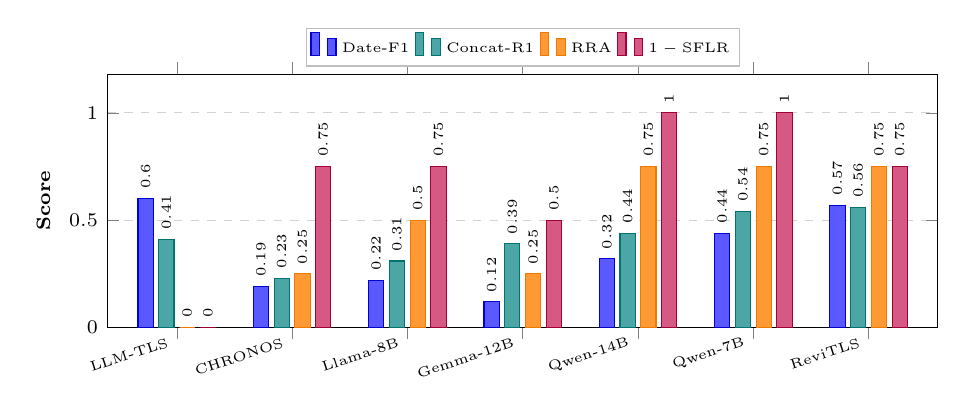
\begin{tikzpicture}
\begin{axis}[
    ybar,
    bar width=5.5pt,
    width=\columnwidth,
    height=4.8cm,
    ymin=0, ymax=1.18,
    ylabel={Score},
    symbolic x coords={LLM-TLS, CHRONOS, Llama-8B, Gemma-12B, Qwen-14B, Qwen-7B, ReviTLS},
    xtick=data,
    x tick label style={font=\tiny, rotate=18, anchor=east},
    y tick label style={font=\scriptsize},
    ylabel style={font=\scriptsize\bfseries},
    legend style={at={(0.5,1.03)}, anchor=south, legend columns=4, font=\tiny, draw=gray!50, inner sep=1.5pt},
    ymajorgrids=true,
    grid style={dashed, gray!35},
    nodes near coords,
    every node near coord/.append style={font=\tiny, rotate=90, anchor=west, /pgf/number format/fixed, /pgf/number format/precision=2}
]
\addplot[fill=blue!65, draw=blue!85!black] coordinates {
    (LLM-TLS, 0.60) (CHRONOS, 0.19) (Llama-8B, 0.22) (Gemma-12B, 0.12) (Qwen-14B, 0.32) (Qwen-7B, 0.44) (ReviTLS, 0.57)
};
\addplot[fill=teal!70, draw=teal!90!black] coordinates {
    (LLM-TLS, 0.41) (CHRONOS, 0.23) (Llama-8B, 0.31) (Gemma-12B, 0.39) (Qwen-14B, 0.44) (Qwen-7B, 0.54) (ReviTLS, 0.56)
};
\addplot[fill=orange!80, draw=orange!95!black] coordinates {
    (LLM-TLS, 0.00) (CHRONOS, 0.25) (Llama-8B, 0.50) (Gemma-12B, 0.25) (Qwen-14B, 0.75) (Qwen-7B, 0.75) (ReviTLS, 0.75)
};
\addplot[fill=purple!65, draw=purple!85!black] coordinates {
    (LLM-TLS, 0.00) (CHRONOS, 0.75) (Llama-8B, 0.75) (Gemma-12B, 0.50) (Qwen-14B, 1.00) (Qwen-7B, 1.00) (ReviTLS, 0.75)
};
\legend{Date-F1, Concat-R1, RRA, $1-\text{SFLR}$}
\end{axis}
\end{tikzpicture}
\caption{Performance comparison across baselines and single/dual-scale ReviTLS backbones on \texttt{T17/bpoil}.}
\label{fig:backbone_chart}
\end{figure}

\begin{table}[t]
\centering
\caption{Ablation Study of ReviTLS Components on \texttt{T17/bpoil}}
\label{tab:component_ablation}
\renewcommand{\arraystretch}{1.12}
\resizebox{\columnwidth}{!}{%
\begin{tabular}{@{}lccccc@{}}
\toprule
\textbf{Model Variant} & \textbf{AR-1} & \textbf{Concat-R1} & \textbf{Date-F1} & \textbf{RRA} & \textbf{Time (s)} \\
\midrule
\textbf{ReviTLS (Full Dual-Scale)} & \textbf{0.081} & \textbf{0.559} & \textbf{0.571} & \textbf{0.750} & \textbf{488.5} \\
\quad w/o Dual-LLM 14B Verifier & 0.079 & 0.553 & 0.550 & \textbf{0.750} & 496.8 \\
\quad w/o Cross-Encoder Reranker & 0.076 & 0.548 & 0.526 & \textbf{0.750} & 512.4 \\
\quad w/o Conditional Temporal Gate & 0.070 & 0.540 & 0.438 & \textbf{0.750} & 619.1 \\
\quad w/o Stale Fact Purging ($\mathcal{P}_k$) & 0.068 & 0.521 & 0.438 & 0.250 & 645.2 \\
\bottomrule
\end{tabular}%
}
\end{table}

\begin{table*}[t]
\centering
\caption{Case Study on the \texttt{T17/bpoil} Stream Comparing the Reference Timeline, LLM-TLS~\cite{hu2024moments}, and \textbf{ReviTLS}. Symbols indicate verified updates/filtering (\checkmark, \textcolor{green!45!black}{\textbf{Green}}) vs.\ leaked stale facts or unretracted rumors ($\times$, \textcolor{red!75!black}{\textbf{Red}}) for black-and-white print compatibility.}
\label{tab:case_study}
\renewcommand{\arraystretch}{1.18}
\resizebox{\textwidth}{!}{%
\begin{tabular}{@{}lp{5.2cm}p{5.5cm}p{5.8cm}@{}}
\toprule
\textbf{Date} & \textbf{Reference Timeline (Ground Truth)} & \textbf{LLM-TLS~\cite{hu2024moments} (Same-Day + TextRank)} & \textbf{ReviTLS (Proposed Dual-Scale)} \\
\midrule
\textbf{2010-04-20} & An explosion and fire occur on the Deepwater Horizon drilling rig in the Gulf of Mexico, leaving 11 workers missing. & An explosion rocks the Deepwater Horizon offshore drilling rig in the Gulf of Mexico, injuring workers and sparking a massive fire. & [\texttt{ACTIVE}] The Deepwater Horizon oil rig explodes and burns in the Gulf of Mexico, with 11 crew members reported missing. \\
\midrule
\textbf{2010-04-22} & The Deepwater Horizon rig sinks; officials later determine oil is leaking at roughly \textbf{5,000 barrels per day} (\texttt{REV-1}). & The Deepwater Horizon sinks into the Gulf; Coast Guard officials estimate the well is leaking [$\times$] \textcolor{red!75!black}{\textbf{1,000 barrels of oil per day}}. & [\texttt{REVISED}] Deepwater Horizon sinks; following NOAA reassessment on Apr~29, the official leak rate is [\checkmark] \textcolor{green!45!black}{\textbf{revised upward to 5,000 barrels per day}} (\textit{1,000 bbl/d purged to $\mathcal{P}_k$}). \\
\midrule
\textbf{2010-05-12} & Congressional investigators examine failed blowout preventer components and \textbf{cement seal failure} (\texttt{REV-3}). & Briefing reports suggest an [$\times$] \textcolor{red!75!black}{\textbf{external seabed shift}} may have triggered the wellhead rupture alongside equipment issues. & [\texttt{REVISED}] Forensic hearings overturn preliminary seabed hypotheses and attribute the blowout to [\checkmark] \textcolor{green!45!black}{\textbf{cementing and shoe-track seal failure}}. \\
\midrule
\textbf{2010-05-20} & \textit{(No valid milestone: May~20 secondary pipeline rupture rumor debunked on May~22, \texttt{REV-4}.)} & [$\times$] \textcolor{red!75!black}{\textbf{Unconfirmed reports indicate a secondary seabed pipeline breach three miles east of the main wellhead.}} & [\checkmark] \textcolor{green!45!black}{\textbf{[RETRACTED \& Filtered]}} \textit{Initial May~20 rumor debunked by ROV sonar inspection on May~22; node excluded from output timeline $\mathcal{T}$.} \\
\midrule
\textbf{2010-05-26} & BP launches the ``top kill'' operation, pumping heavy drilling mud into the ruptured blowout preventer. & BP engineers begin the ``top kill'' procedure, injecting heavy drilling fluids into the crippled wellhead to stem the oil flow. & [\texttt{ACTIVE}] BP initiates the ``top kill'' operation, pumping heavy drilling mud into the blowout preventer to halt the leak. \\
\bottomrule
\end{tabular}%
}
\end{table*}

\subsection{Multi-Model Analysis and Ablation Study}
\label{subsec:ablation}

Table~\ref{tab:ablation_study} and Fig.~\ref{fig:backbone_chart} evaluate the impact of LLM scale and attention mechanisms across four backbones:
\begin{enumerate}
    \item \textbf{Cross-Date Over-Merging Across Model Scales:} Under an unconstrained 90-day lookback window, scaling from \texttt{Qwen2.5-7B} ($\text{Date-F1}=0.438$) to \texttt{Qwen2.5-14B} ($\text{Date-F1}=0.316$) or \texttt{Gemma-3-12B} ($\text{Date-F1}=0.118$) reduces temporal precision. Larger models exhibit broader semantic associativity, frequently classifying subsequent daily milestones in a single-topic stream as \texttt{UPDATE\_PROGRESS} of earlier clusters rather than \texttt{NEW\_EVENT}. Restricting routine events to same-day matching via Eq.~\eqref{eq:temporal_gate} while routing only revision-cued events to the $14\text{B}$ verifier resolves this bottleneck ($\text{Date-F1} = \mathbf{0.571}$).
    \item \textbf{Effect of Attention Mechanism:} Models using full Dense GQA (\texttt{Qwen2.5-7B/14B}) achieve superior revision accuracy ($\text{RRA} = 0.750$) compared to \texttt{Gemma-3-12B}'s 5:1 Local-Global Sliding Window Attention ($\text{RRA} = 0.250$), which struggles with multi-slot JSON adherence and cross-date conflict detection.
    \item \textbf{Component Ablation and Inference Efficiency:} Table~\ref{tab:component_ablation} shows the contribution of each module. Removing stale fact purging ($\mathcal{P}_k$) drops $\text{RRA}$ from $0.750$ to $0.250$. Removing the Conditional Temporal Gate drops $\text{Date-F1}$ from $0.571$ to $0.438$ and increases inference time from $488.5\text{s}$ to $619.1\text{s}$. Overall, our two-phase dual-LLM schedule reduces runtime by $\mathbf{21.1\%}$ compared to single-scale $7\text{B}$ ($619.1\text{s}$) and by $\mathbf{30.8\%}$ compared to single-scale $14\text{B}$ ($706.3\text{s}$) by filtering non-revision candidates before cross-date LLM verification.
\end{enumerate}

\subsection{Case Study}
\label{subsec:case_study}

Following the qualitative evaluation protocols of LLM-TLS~\cite{hu2024moments} and CHRONOS~\cite{wu2025unfolding}, Table~\ref{tab:case_study} presents a side-by-side comparison of partial timelines generated on the \texttt{T17/bpoil} stream. On April~22 (\texttt{REV-1}), six early articles report an initial leak estimate of ``1,000 barrels per day.'' When NOAA releases its official revision of ``5,000 barrels per day'' on April~29 ($\Delta t = 7$~days later), LLM-TLS cannot link the April~29 article to the April~22 cluster due to its same-day filter, leaving the outdated figure in the summary. In contrast, ReviTLS detects the revision cue ($\rho_{i,j}=1$), matches the April~22 state via Cross-Encoder reranking ($S_{\text{hyb}}=0.89$), purges ``1,000 barrels per day'' into $\mathcal{P}_k$, and updates the milestone to ``5,000 barrels per day'' (\texttt{REVISED}). Similarly, on May~20 (\texttt{REV-4}), when a breaking rumor of a secondary pipeline breach is debunked by ROV sonar inspections on May~22, LLM-TLS retains the false rumor as a standalone milestone, whereas ReviTLS transitions the node to \texttt{RETRACTED} and excludes it from the final timeline.

\section{Conclusion}
\label{sec:conclusion}

We presented \textbf{ReviTLS}, a revision-aware two-phase timeline summarization framework designed for non-monotonic news streams. By modeling events as mutable $5\text{W}1\text{H}$ state nodes with tombstone purging, a Conditional Dual-Horizon Temporal Gate, cross-encoder reranking, and deferred $14\text{B}$ conflict verification, ReviTLS resolves cross-date factual revisions and rumor retractions while mitigating cross-date milestone over-merging. Across $13$ T17 and Crisis topics, ReviTLS improves content coverage and alignment on T17 under identical hardware conditions while resolving $81.3\%\text{--}87.5\%$ of controlled multi-topic revisions and $100\%$ of counterfactual controls with zero pre-correction leakage, at the cost of higher inference latency than single-pass clustering baselines.

\subsection{Limitations and Future Work}
\label{subsec:limitations}

Our study has five primary limitations that motivate future work:
\begin{enumerate}
    \item \textbf{Computational Overhead:} Structured $5\text{W}1\text{H}$ extraction and $14\text{B}$ conflict verification make ReviTLS roughly $3.9\text{--}4.5\times$ slower than same-day LLM-TLS; its two-phase schedule minimizes GPU model swaps but defers Phase~2 revisions until stream end rather than emitting fully revised states strictly online.
    \item \textbf{Cue Reliance and Irreversible Retraction:} The Conditional Temporal Gate relies on lexical/structural cues ($\rho_{i,j}=1$) and may miss purely implicit corrections; conversely, false-positive \texttt{RETRACTED} transitions permanently suppress valid milestones.
    \item \textbf{Synthetic Suite Scope and Sample Size:} Standard TLS corpora lack native revision histories; our $16$-scenario and $8$-scenario suites are author-constructed over $\Delta t \in [2, 8]$~days, and the $9$-topic T17 sample limits statistical power under multiple-comparison correction.
    \item \textbf{Corpus Age and Language:} T17 and Crisis contain English news from 2005--2013; evaluating multilingual streams and post-cutoff recent events remains open.
    \item \textbf{Automated Evaluation:} While we use standard Tilse metrics and automated state/claim verification, large-scale human evaluation and natively human-annotated non-monotonic timeline corpora are important directions for future work.
\end{enumerate}

\bibliographystyle{IEEEtran}
\bibliography{references}

\end{document}
